\documentclass[tikz,border=2pt]{standalone}
\usepackage{amsmath,amssymb}
\usepackage{pgfplots}
\pgfplotsset{compat=1.18}
\usetikzlibrary{arrows.meta}
\begin{document}
% Grouped exponential losses: bins (0,100] and (100,inf) with counts 6 and 4. The bin probabilities are
% p_1 = 1 - e^{-100 lambda}, p_2 = e^{-100 lambda}; at the maximizer lambda = log(2.5)/100 they equal 0.6 and 0.4.
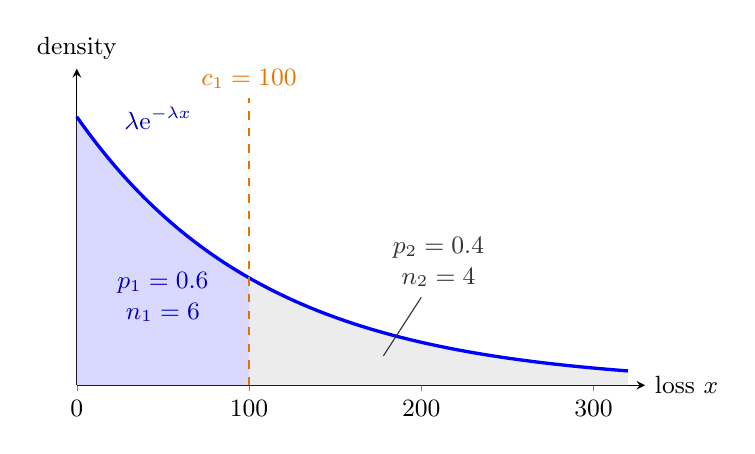
\begin{tikzpicture}[font=\small, >={Latex[length=2mm]}]
  \begin{axis}[
    axis lines=left, xmin=0, xmax=330, ymin=0, ymax=0.0108,
    xtick={0,100,200,300}, ytick=\empty,
    xlabel={loss $x$}, ylabel={density},
    xlabel style={at={(axis description cs:1,0)}, anchor=west},
    ylabel style={rotate=-90, at={(axis description cs:0,1)}, anchor=south},
    width=8.8cm, height=5.6cm, clip=false
    ]
    \def\lam{0.0091629}
    \addplot[fill=blue!15, draw=none, domain=0:100, samples=40] {\lam*exp(-\lam*x)} \closedcycle;
    \addplot[fill=gray!15, draw=none, domain=100:320, samples=60] {\lam*exp(-\lam*x)} \closedcycle;
    \addplot[blue, very thick, domain=0:320, samples=100] {\lam*exp(-\lam*x)};
    \draw[orange!90!black, thick, dashed] (axis cs:100,0) -- (axis cs:100,0.0098);
    \node[orange!90!black, anchor=south] at (axis cs:100,0.0098) {$c_1=100$};
    \node[blue!70!black, align=center] at (axis cs:50,0.0030) {$p_1=0.6$\\$n_1=6$};
    \node[gray!40!black, align=center] at (axis cs:210,0.0042) {$p_2=0.4$\\$n_2=4$};
    \draw[gray!40!black, thin] (axis cs:200,0.0030) -- (axis cs:178,0.0010);
    \node[blue!70!black, anchor=south west] at (axis cs:22,0.0084) {$\lambda \mathrm{e}^{-\lambda x}$};
  \end{axis}
\end{tikzpicture}
\end{document}
